\section{Results and Discussions}
\begin{figure*}[!t]
    \centering
    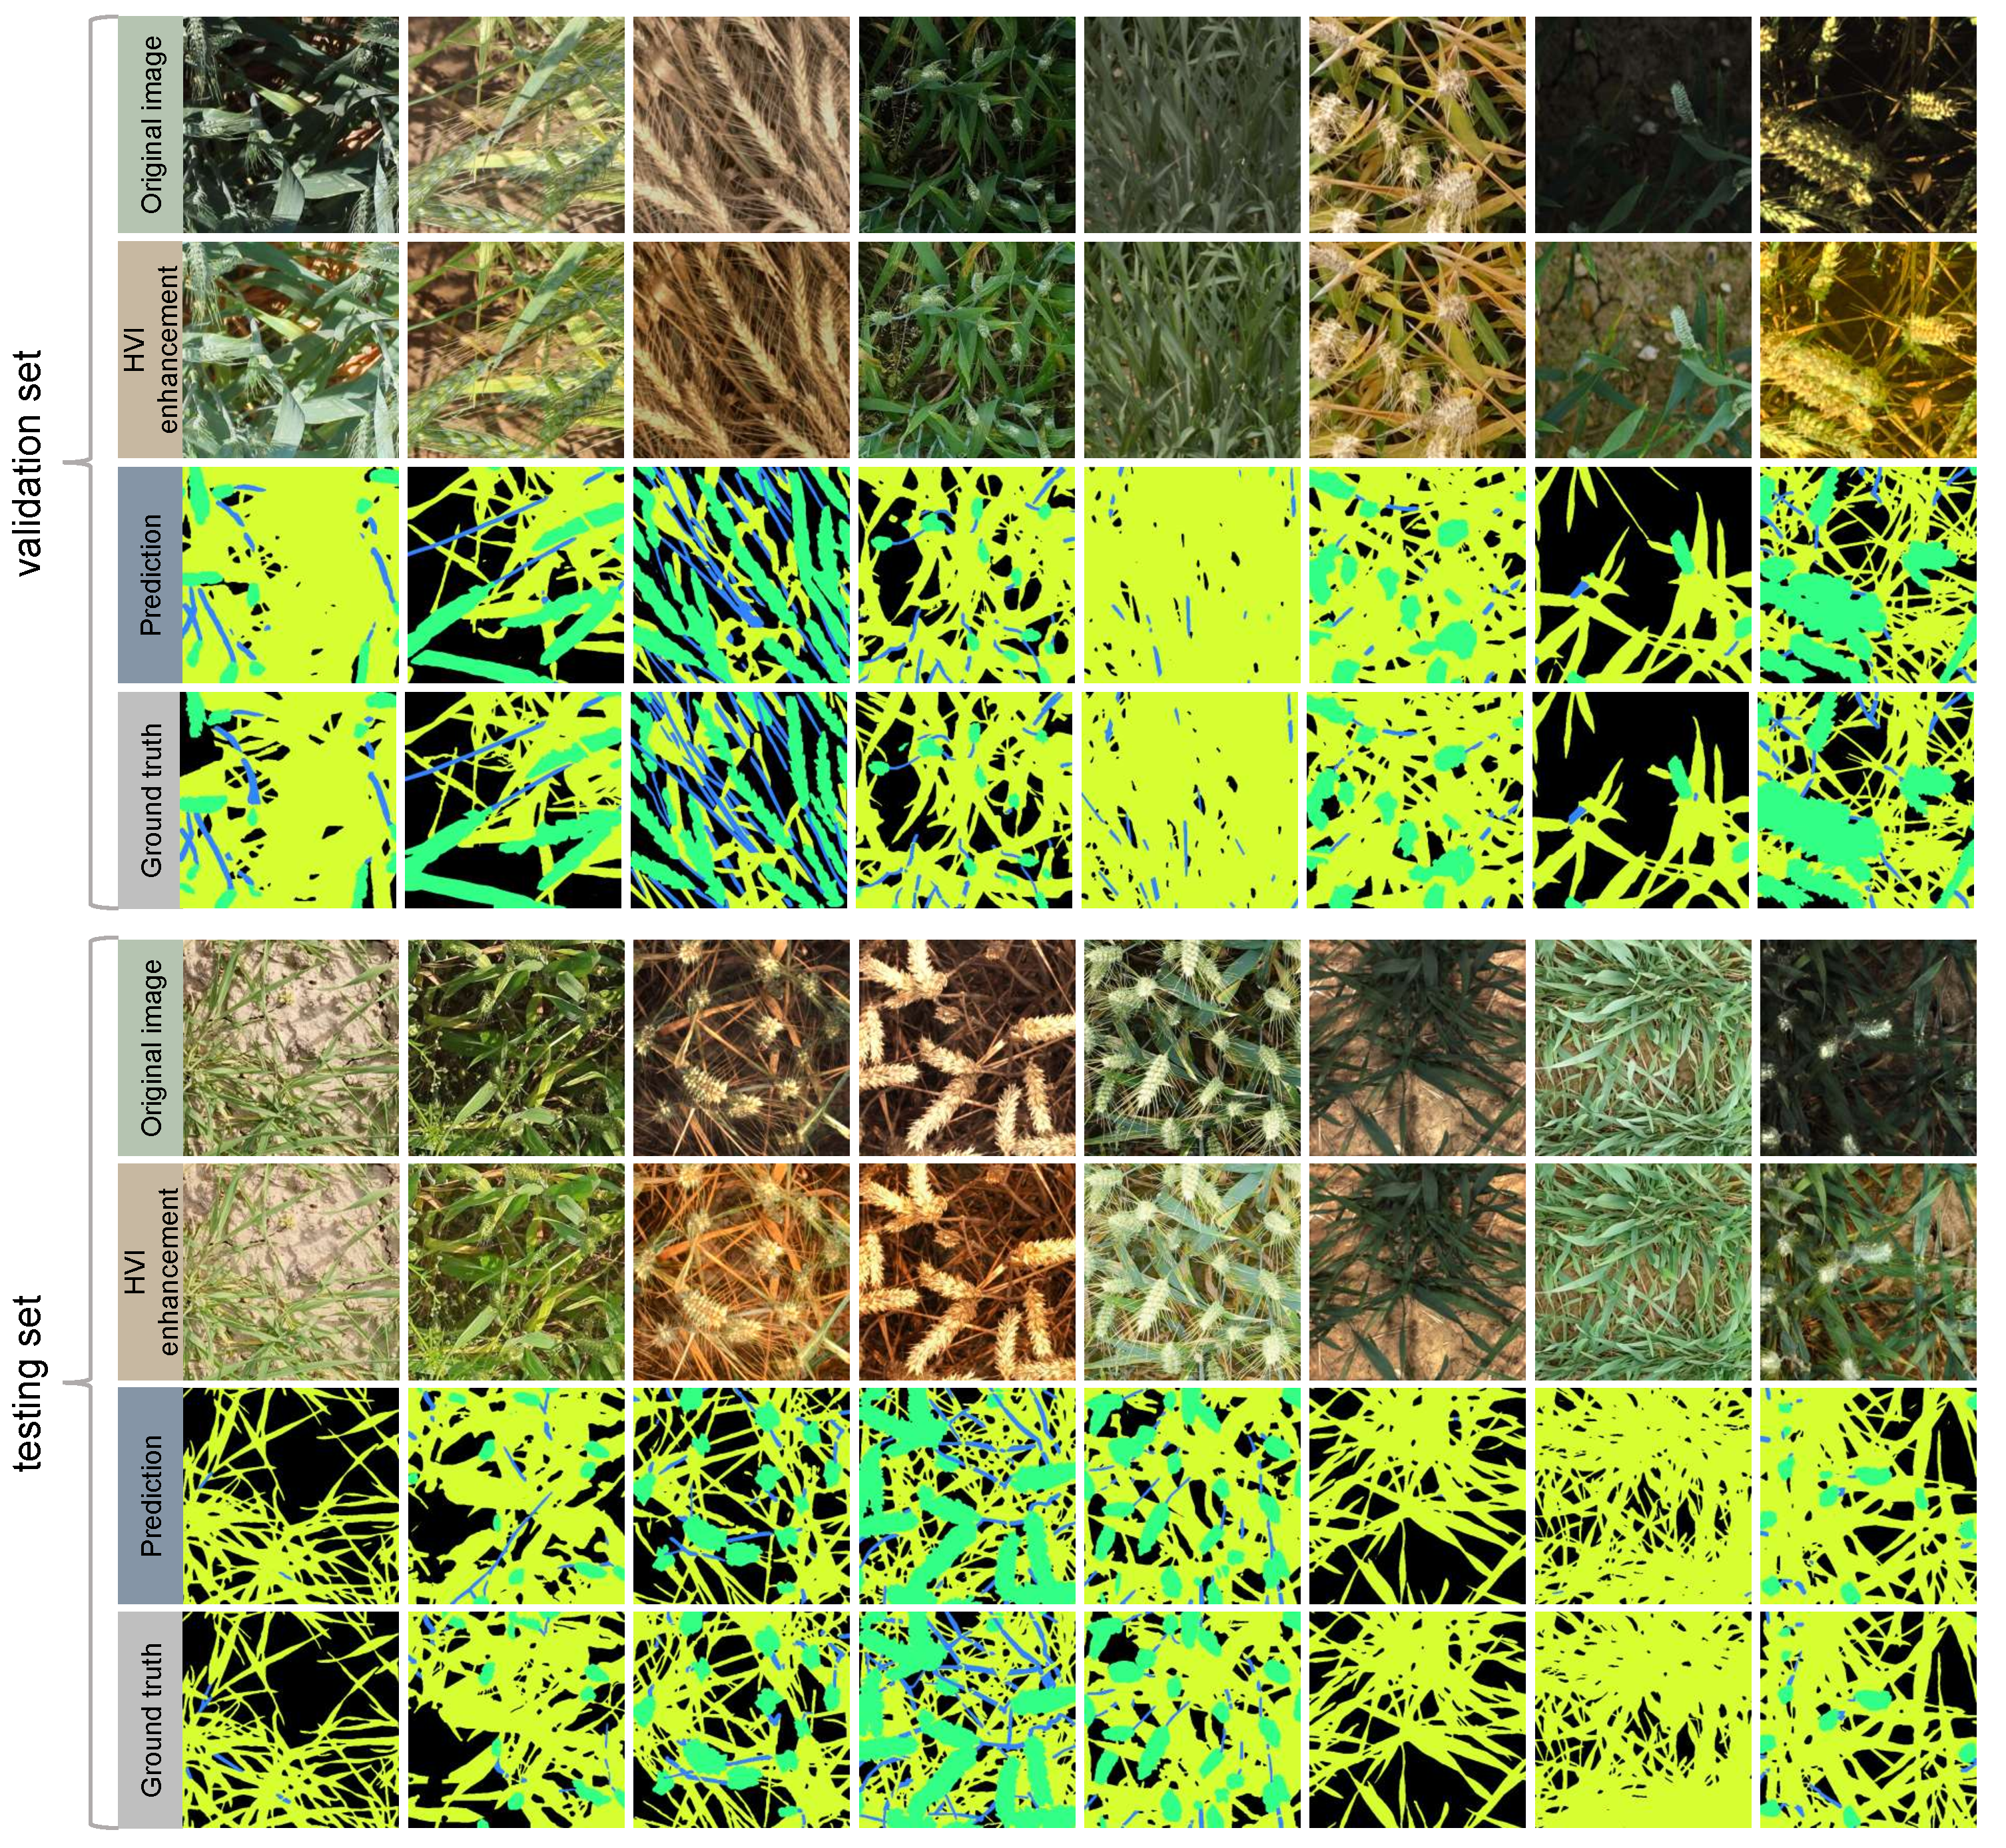
\includegraphics[width=\linewidth]{val_test_vis.pdf}
    \caption{\textbf{Visualization of our model on validation and testing set}.}
    \label{fig:val_test_vis}
\end{figure*}
Here we present our results and discussions. Before that, we first introduce the evaluation metric used and our implementation details.

\subsection{Evaluation Metric}
The evaluation metric % used in the competition is 
follows the standard semantic segmentation metric, that is, the mean Intersection over Union (mIoU), which is defined by
\begin{equation}
    \text{mIoU}=\frac{1}{N}\sum_{i=0}^N\frac{\text{TP}_i}{\text{TP}_i+\text{FP}_i+\text{FN}_i}\,,
\end{equation}
where $N$ is the number of classes. TP, FP, and FN denote the number of true positives, false positives, and false negatives for each class, respectively.

\subsection{Implementation Details}
We use the ImageNet-1K pretrained weight of BEiTv2-Large from the official repository, which has first trained for $1600$ epochs in a self-supervised manner and then finetuned for another 50 epochs following supervised learning. During our supervised learning stage for training a segmentation model, the model is trained for $20$K iterations, with a batch size of $16$. The base learning rate is set to $0.0001$, and the backbone learning rate is $0.01$. We use the ploy LRScheduler and set the warm up iterations to $0$. % This training 
The first stage % typically 
takes approximately 5 hours to complete. In the guided distillation stage, we set the total iterations to $90$K, with $20$K iterations for guided burn-in stage and apply early stop strategy. This stage requires about three days of training time. For the loss weights, we set $\lambda_{dice}=5$, $\lambda_{c}=5$, and $\lambda_u=2$. The EMA decay rate $\alpha$ is set to $0.9996$. In the testing stage, we use scaling ratios $\S=\{1.0, 1.5, 2.0, 2.5, 3.0, 3.5\}$ to scale the input image and apply sliding inference for each image. All experiments are conducted on the Ubuntu 20.04 system and on a workstation with four $48$ GB RTX A6000 GPUs, two $10$-core Intel Xeon Silver 4210R CPUs, and $256$ GB RAM.

\begin{table}[!t]
    \centering
    \begin{tabular}{@{}lc@{}}
    \toprule
       \textbf{Testing Scale}  &  \textbf{Leaderboard Score}\\
    \hline
        $512$ & $0.74$ \\
        $768$ & $0.76$ \\
        $512,768,1024,1280,1536,1792$ & $0.77$ \\
    \bottomrule
    \end{tabular}
    \caption{\textbf{Scores with different test-time scaling configurations}. Through the strategy of \textit{zoom in and segment twice}, we achieved a significant improvement. While extend our startegy to multi-scales, we can improve the performance further.}
    \label{tab:test_time_scale}
\end{table}



\begin{table}[!t]
    \centering
    \scalebox{0.87}{
    \begin{tabular}{@{}lcc@{}}
    \toprule
        \textbf{Team Name} & \textbf{Development Phase} & \textbf{Testing Phase} \\
    \hline
        HUST\_TinySmart (Ours) & $\textbf{0.77}$ & $\textbf{0.75}$  \\
        ZR Yang\&JH Jiang & $0.75$ & $0.71$  \\
        good & $0.75$ & - \\
        tapu1996 & $0.74$ & n/a \\
        pcccl & $0.74$ & $0.7$ \\
        willer & $0.74$ & - \\
        asuka & $0.74$ & $0.69$ \\
        nncckkuu & - & $0.68$ \\
        enchanter & $0.71$ & $0.66$ \\
        zaorui\_njfu & $0.71$ & $0.65$ \\
        Dafang Zou & $0.71$ & - \\
        tiezhuma & $0.7$ & $0.64$ \\
        phasheen & $0.69$ & - \\
        jaykk & $0.69$ & - \\
        xmba15 & $0.69$ & $0.63$ \\
        dsvolkov & $0.66$ & $0.62$ \\
        zengyangche & $0.67$ & $0.61$ \\
        perrychen & $0.64$ & - \\
        HZAU AISLE Group & $0.63$ & $0.57$ \\
        loannis Droutsas & $0.57$ & $0.54$ \\ 
        
    \bottomrule
    \end{tabular}}
    \caption{\textbf{Official leaderboard scores}. Top 20 teams from the development phase only (as of June 21, 2025). The scores are rounded mIoU.}
    \label{tab:leaderboard_score}
\end{table}

\subsection{Main Results}
The effect of our different stages in the development phase can
be found in Table~\ref{tab:ablation}. % Although our baseline has already achieved strong performance, there is still room for further improvement. As shown in Fig.~\ref{fig:sapa_baseline}, the SAPA-Enhanced ViT-Adapter model produces smoother segmentation edges than baseline and achieves a certain improvement in mIoU. 
Results justify that each our design choice makes a difference. Surprisingly, the test time scaling stage yields the most significant improvement, improving the stage-two model by 0.0272 scores. A plausible explanation is that the model can better sense the detail of the stem class when zooming in the image. % the improved consistency between the training and testing phases enabled by this method. % In stage-two training, we apply different data augmentations (\eg, random resizing, random cropping, and color enhancement). Thus, during testing, the model can better recognize the input image and handle small class by "zoom in and segment". % Although SAPA dynamic upsampling operator makes few improvement, it can enable the model to produces smoother segmentation edges than basline.  
% Unlike using all the unlabeled data to pre-train a vision backbone, we choose to apply the semi-supervised pipeline. 
We also test the effect of different scaling ratios. The scores can be found in Table~\ref{tab:test_time_scale}. It can be observed that the single-scale zoom-in operation brings the most significant improvement. While our final solution uses the multi-scale inference strategy (segment twice), it introduces significant computational cost. 

The final competition results of the development and testing phases are shown in Table~\ref{tab:leaderboard_score}. Through our three improvements, we finally achieve a score of $0.7704$ in the development phase and $0.7468$ in the testing phase. Our solution ranks the first place on both the development and testing leaderboard. Remarkably, it exhibits the least performance drop in the testing phase, indicating strong generalization of our solution. % superior robustness of our approach. 
In our view, this is mainly attributed to guided distillation, which enhances the training robustness of the model. Although our three improvements seem to be simple, we believe the key to our success is to follow the philosophy of the devil is in the detail and minority, that is, the \texttt{stem} class. The qualitative results of our final model are shown in Fig.~\ref{fig:val_test_vis}. % Our trained model shows a robust performance in the data outside the domain.
% Our model produces predictions with good detail delineation and coherent region prediction.


